\documentclass[a4paper,12pt]{article}
\usepackage{a4wide}
\usepackage{acronym}
\usepackage{graphicx}
\usepackage[title,titletoc,toc]{appendix}


\begin{document}

\begin{center}
{\LARGE\bf Travelling Thief Problem}\\
\vspace{0.5cm}
{\Large\bf Evolutionary Computation}\\
\vspace{1cm}
Prepared by William Reid, Matthew Hart, Samantha Peachey \& Alec Bellati\\
\vspace{1cm}
School of Computer Science,\\
The University of Adelaide\\
\vspace{1cm}
\today
\end{center}

\vspace{1cm}
\section*{Exercise 2}
This exercise focuses on modifying only the packing of the knapsack - the TSP tour is supplied in a text file that is read-in using the \textit{linkern tour} method provided in the \textit{Optimisation} class. Since this problem revolves around solving the traditional knapsack problem, research into solutions suggested a purely evolutionary approach may yield good results in the appropriate time-frame, however there was little guarantee it would obtain the optimal result. As such, the following solution is evolved from a purely linear approach which I have labelled - Obsessive Packing.

\section{Obsessive Packing}
This algorithm performs 3 fundamental steps, 2 of which are repeated a number of times.
\begin{enumerate}
	\item Seed the knapsack with items using various methods
	\item Evaluate the solution and remove any unnecessary items
	\item Take every item not in the knapsack and for each item:
		\begin{itemize}
			\item Directly add the item to the knapsack (if weight will not be exceeded) and evaluate the result. If the result is better, skip the next step.
			\item One at a time, temporarily replace every item in the knapsack with the current item (if weight will not be exceeded). Evaluate the result for every replacement and once complete - if a better result can be obtained, permanently replace an item (optimal position now obtained) in the knapsack with the current item.
		\end{itemize}
 \end{enumerate} 

\newpage

Steps two and three listed above can be performed multiple times to further the result of the knapsack. The diagram below illustrates how step 3 is performed. It iteratively performs this step over every item in the knapsack, ensuring that the item will be placed in the most optimal position. The final placement (if one is found) permanently modifies the current knapsack. If at the end of the evaluation period the item does not have an optimal position, it is not added to any position in the knapsack.
\begin{figure}[h]
\centering
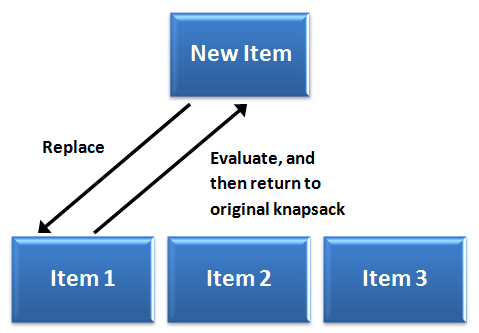
\includegraphics{ObsessivePacking.png}
\end{figure}

\subsection{Profit Evaluation}
The evaluate the profit of the solution at each step, the \textit{evaluate} function from the TTPInstance class was used. This ensures that the calculated profit uses the correct formulas and also reduces the code base. Research was done into faster evaluation methods and while it is possible to create a simpler (but less accurate) evaluation technique, the gains were not significant enough for the implementation of a new method.

\subsection{Useability on Problem Types}
The primary bonus in the choice of this algorithm is it ensures it will behave in similar ways, no matter how the problem is presented. Whether it be strongly bounded, uncorrelated, single item per city, multiple items per city or thousands of cities - the algorithm will be able to obtain good results. The reason for this is its seperate stages of addition, removal and replacement of items, which benefits selective types of data sets. While this process may perform some unecessary operations, it ensures it can be used on a broad range of problem types.


\newpage
\section{Modifications for Larger Data Sets}
\subsection{Item Subset}
Since the algorithm considers all items not in the knapsack, it has the potential to grow so large that it may not process important items within the allowable runtime. As a result, for the larger data sets (pla33810) the algorithm only considers a subset of items not contained in the knapsack. The number of items is specific to the problem size but these instances only consider between 2500 and 10000 items that are currently not in the knapsack. These items are approximately 75\% of the ``best'' items and the remaining 25\% are randomly chosen. The ``best'' items are chosen based on their profit-to-weight ratio.

\subsection{Item Replacement}
Replacing all items in the knapsack greatly increases the runtime. Similar to the section above, the larger data sets may produce large knapsacks and hence replacing every item in the knapsack may reduce the number of items that can be considered. To combat this, the larger data sets are given a maximum number of ``iterations''. An iteration is where an item in the knapsack is replaced with the current item and evaluated (see previous diagram). Where the smaller data sets consider the entire knapsack, the larger data sets may only consider 5 or 15 items to replace in the knapsack. 

\section{Testing and Additional Methods}
Various methods were employed to better the result of the solution. These included:
\begin{itemize}
	\item Methods to seed the knapsack in different ways
	\item Intelligent methods for selecting subsets of items
	\item Additional methods for modifying the TSP (not considered for this exercise)
	\item Heuristics for selecting the optimal items to replace in the knapsack
\end{itemize}

While these methods served as useful tests and concepts, they did not prove profitable within the algorithm. These methods can be found at the bottom of the algorithm implementation, still available for use.

\newpage
\subsection{Parameter Tweaking}
The Obsessive Packing algorithm relies on the parameters defined below. While a baseline set of parameters can be supplied, the algorithm works best when these values are ``tweaked'' for the specific data set.
\begin{itemize}
	\item {\bf Knapsack Seed:} The algorithm allows for various methods to seed the knapsack. The ``seed'' is the starting packing of the knapsack and can greatly affect the final result.
	\item {\bf TSP Choice:} To account for extendibility, this algorithm not only considers just the packing of the knapsack, but may also consider changes to the TSP tour.
	\item {\bf Generations:} Number of times to perform the algorithm on the knapsack (knapsack packing is retained for the next generation, it is not re-seeded).
	\item {\bf Iterations:} Number of times to replace a randomly chosen item in the knapsack with the current item.
	\item {\bf Items to be considered:} Number of items to be placed in the knapsack to evaluate.
\end{itemize}

\section{Conclusion}
While this algorithm does prove computationally intensive, it does provide intelligent heuristics to adequately remove data that is considered unusable. While this algorithm is best used by tweaking a number of its values (explained in the testing section), it can be run with a general set of parameters, over various types of data sets, and still obtain good results. Initial runs with this algorithm prove its results are better than those obtained using the supplied \textit{Hill Climber} algorithm. Further explanation of these results can be found in Exercise 5.\\

To better the usage of this algorithm, methods to intelligently select what items need replacing within the knapsack would reduce computation and may also allow for more items to be considered in larger data sets. In addition, methods to modify the parameters explained in the testing section would also allow for greater results and relinquish the need for the user to optimise the parameters. It would also ensure that operations best suited to that data set are used more often and more efficiently - for instance the larger data sets benefit from removing as many items as possible and them replacing very few with some good quality items.\\

Finally, a more approximation based profit evaluation method may reduce computation time. As the instances become larger it takes a considerable amount of time to evaluate each solution, especially when it is done multiple times for each item not contained within the knapsack.


\end{document}
